\chapter{Análise Bibliográfica sobre Criptografia no Universo da Computação Quântica, por André Larrosa Chimpliganond}

\section{Planejamento do estudo}
Como se transmitir informações de modo que esta só possa ser acessada pela pessoa certa? Responder essa pergunta e elaborar métodos para por a solução em prática é área de estudo da criptografia. Utilizando de alta complexidade matemática, técnicas de criptografia codificam informações de modo que só possam ser decodificadas por quem possuir a chave. Mas como o advento e evolução da computação quântica afeta a maneira como criptografamos os dados?

Partindo dessa pergunta, podemos explorar outras que irão nortear o trabalho:
\begin{itemize}
    \item Quais conceitos relacionados à esse embate entre a criptografia e computação quântica?
    \item Quais autores, instituições e nações estão à frente desse tema?
    \item Como esse conteúdo tem se desenvolvido ao longo do tempo?
\end{itemize}



% nao sei se vou colocar
\subsection{O que já existe de pesquisa bibliométrica sobre esse tema?}

\cite{gore_classifying_2016} fizeram uma pesquisa que visava aprofundar a questão da simulação multiagente em relação à computação experimental.

A pesquisa é base para um posterior aprofundamento no campo da Cientometria, como fez \cite{chavalarias_whats_2017}.
% 

\subsection{Ferramentas}
Será utilizada a interface web para o pacote Bibliometrix (Biblioshiny). O pacote Bibliometrix é uma ferramenta R que fornece um conjunto de ferramentas para a investigação quantitativa em cientometria e bibliometria.


% nao sei se vou colocar
\subsection{Limitações} O exercício relatado foi feito em uma semana, envolvendo entre 5 a 10 horas de trabalho de cada autor.

Outros aspectos a reforçar:
\begin{itemize}
   
\item Deve-se fazer buscas na base de dados WoS ou SCOPUS;
\item é obrigatório declarar um conjunto de perguntas de pesquisa.
\item é preciso declarar o objetivo da pesquisa, que no caso da aqui relatada foi exercitar inicialmente, e relatar, o uso da técnica de análise bibliométrica, para fins didáticos.
\end{itemize}
%

\section{Coleta de dados}%label

A coleta de dados feita usando o Web Of Science  no dia 09 de fevereiro de 2022, acessado por meio do Portal de Periódicos da CAPES.

Foram feitas buscas nas coleções \textbf{Science Citation Index Expanded (SCI-EXPANDED)--1945-presente}, \textbf{Conference Proceedings Citation Index – Science (CPCI-S)--1990-presente} e \textbf{Emerging Sources Citation Index (ESCI)--2017-presente}. 

Foi usada a seguinte \query\  de busca

\lstinputlisting[numbers=left,basicstyle=\normalsize\ttfamily,caption={\query\  de busca sobre criptografia quântica.}]%label
{experiments/andrelarrosacrypt/AnaliseBibliometrica/CriptografiaQuantica/query.txt}

\subsection{Explicação para os termos de busca usados}%label

Foram elaboradas duas cláusulas de busca unidas por \textit{and}. A primeira foca nos elementos relacionados ao universo quântico, enquanto a segunda faz referência à criptografia.


Os 10522 registros obtidos encontram-se no github do projeto, em \url{https://github.com/jhcf/Comput-Experim-20212/experiments/andrelarrosacrypt/AnaliseBibliometrica/CriptografiaQuantica/rec_1.txt} e \url{https://github.com/jhcf/Comput-Experim-20212/experiments/andrelarrosacrypt/AnaliseBibliometrica/CriptografiaQuantica/rec_2.txt}. 
% enviar arquivo completo direto no overleaf

Foram exportadas todas as informações disponíveis na Web Of Science de cada documento

\section{Análise dos dados}

\subsection{Filtragem de registros}


Após carregar o dataset na plataforma biblioshiny, foi feita uma filtragem dos documentos com o intuito de selecionar apenas os artigos publicados em revistas científicas (\textit{ARTICLE}). Após a filtragem, sobraram 7131 documentos. Esse novo dataset será nomeado CriptografiaQuanticaArtigos ou CQA@andrelarrosacrypt.

\subsection{Informações principais do \dataset\   CQA@andrelarrosacrypt}
\begin{description}
    \item[Período]	1988 - 2022
    \item[Fontes]	675
    \item[Documentos]	7131
    \item[Média de tempo de publicação]	8.31
    \item[Média de citações por documento]	33.05
    \item[Média de citações por ano por documento]	2.75
    \item[Referências]	83981
    \item[Palavras-chave (Keywords Plus (ID))]   3187
    \item[Palavras-chave (Author's Keywords (DE))] 8201
    \item[Autores]   10925
    \item[Aparições de autores]	28034
    \item[Autores de documentos de autoria única]	436
    \item[Autores de documentos de autoria múltipla]	10489
    \item[Documentos de autoria única]	706
    \item[Média de documentos por autor]	0.653
    \item[Média de autores por documento]	1.53
    \item[Média de co-autores por documento]	3.93
    \item[Index de colaboração (Autores de documentos de autoria múltipla/Docuemntos de autoria múltipla)]        1.63
\end{description}


\subsection{Evolução da Produção Científica}

\begin{figure}
    \centering
    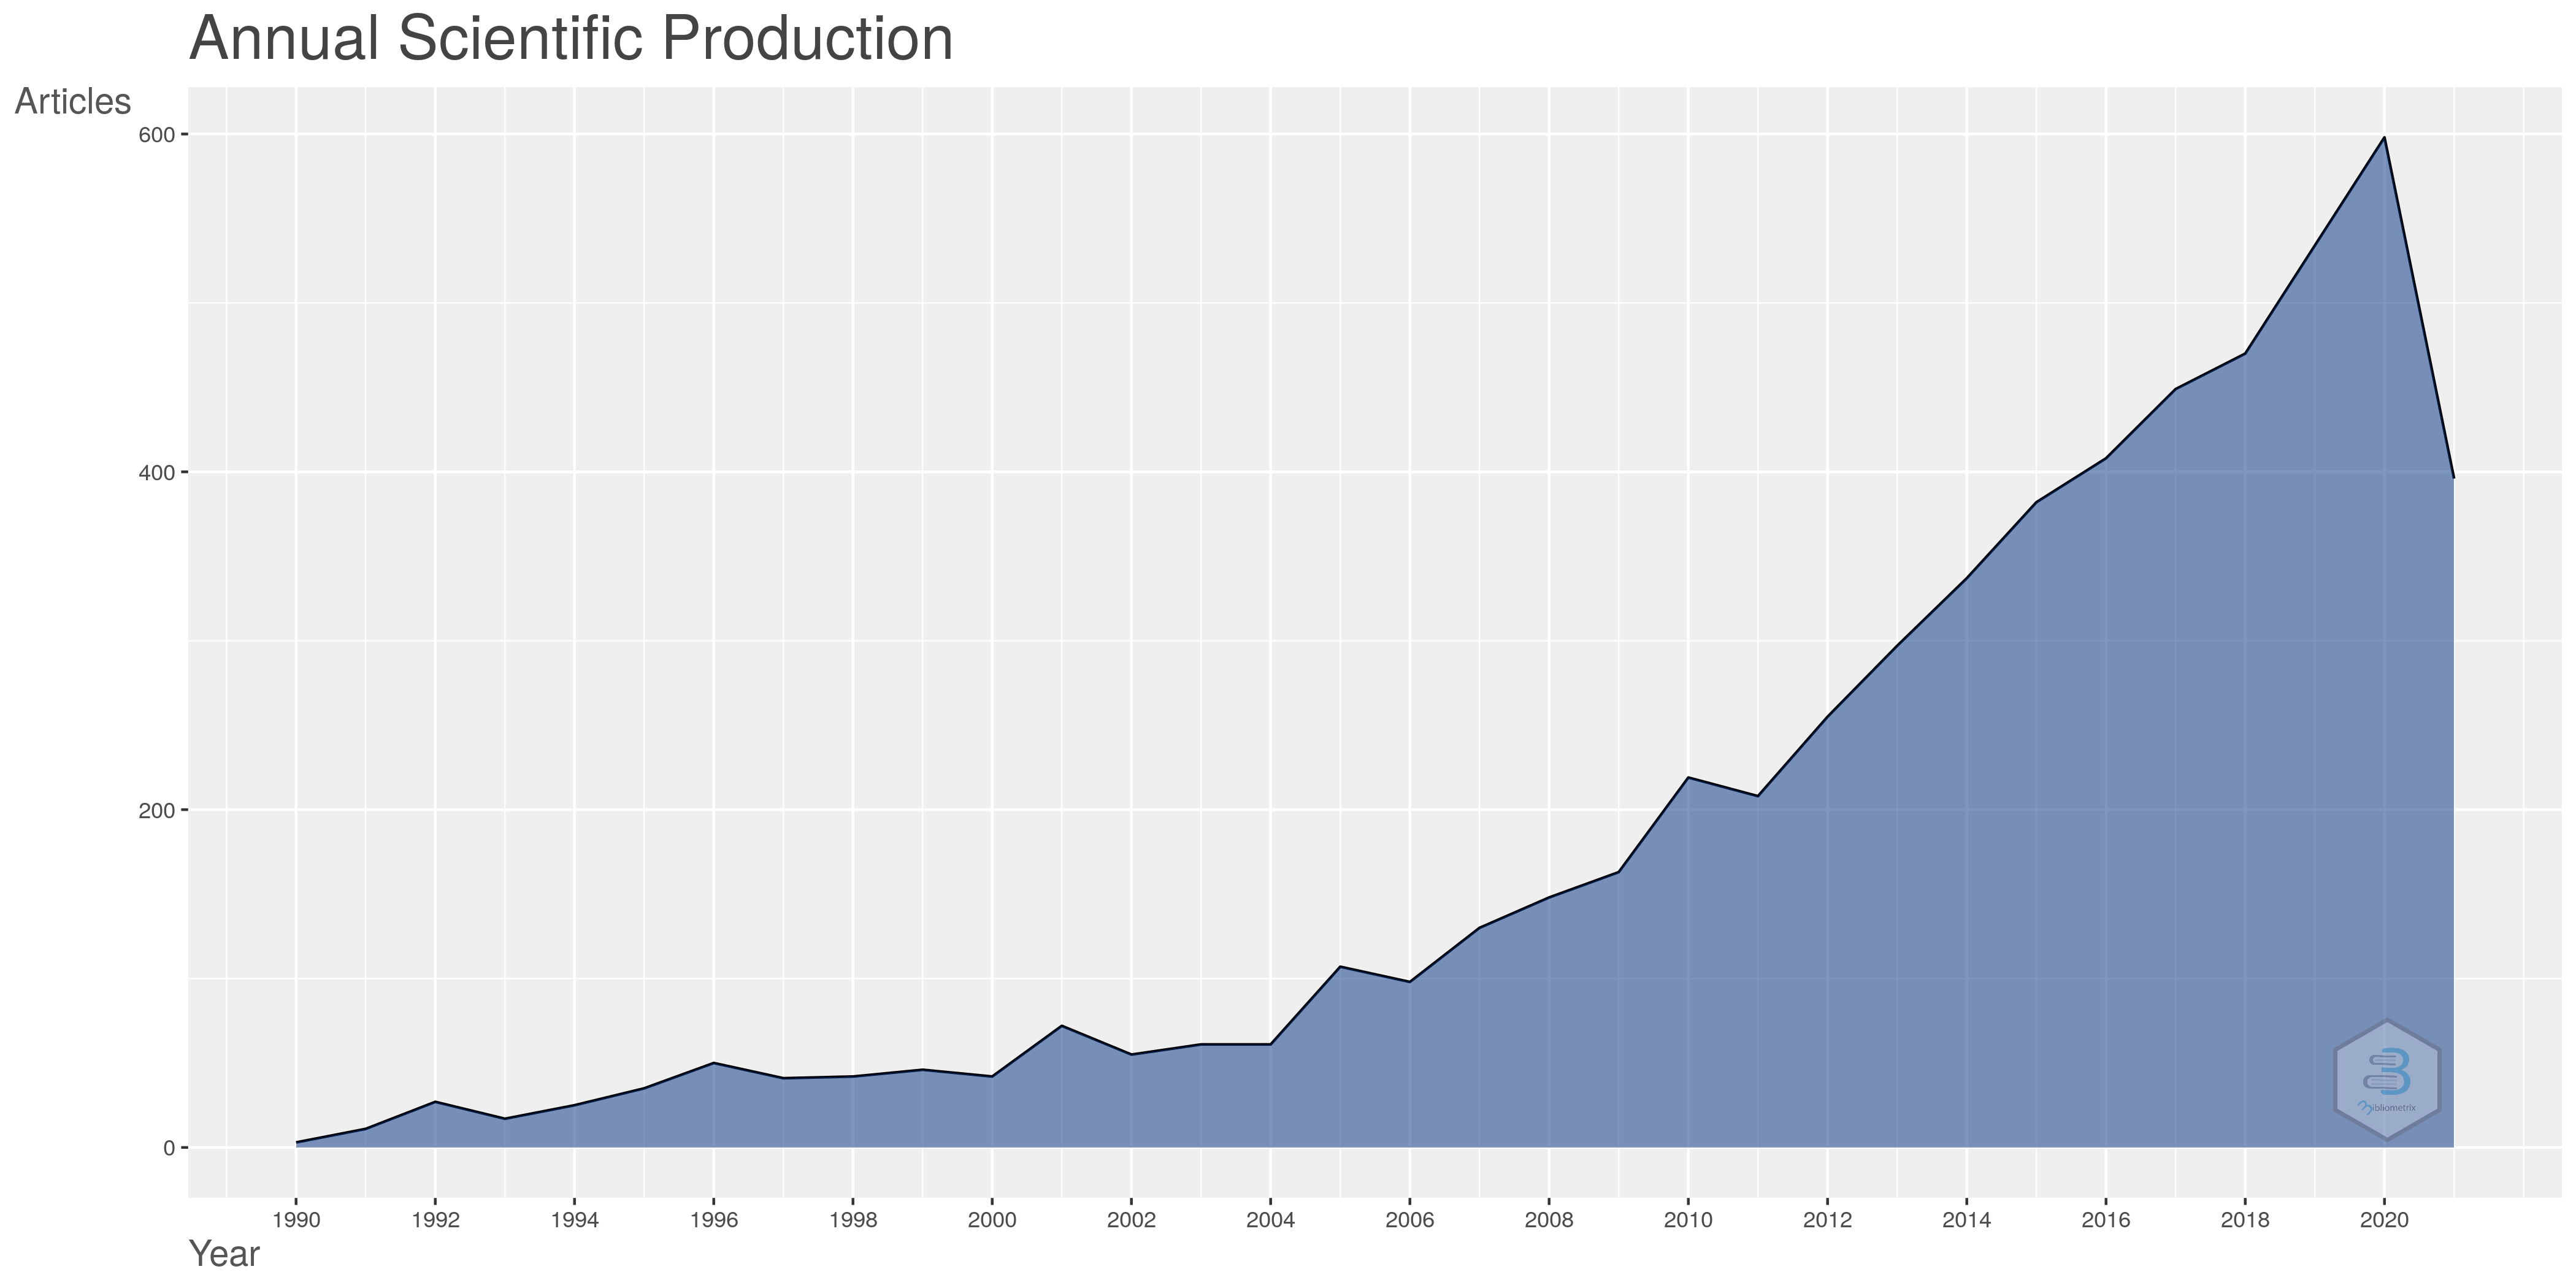
\includegraphics[width=1\textwidth]{experiments/jhcf/PesqBibliogr/SimulacaoMultiagente/WoS-20210803/classico-mais-citacoes/Dataset/AnnualScientificProduction-2021-08-05.png}
    \caption{Evolução da produção científica no \dataset\   MASSA@jhcf.}
    \label{fig:evol:anual:MASSA@jhcf}
\end{figure}

A figura \ref{fig:evol:anual:MASSA@jhcf} apresenta a evolução da produção científica mundial no tema de interesse, segundo o \dataset\   MASSA@jhcf. A curva mostra uma tendência de crescimento aproximadamente exponencial da quantidade de publicações, desde a primeira identificada em 1990.

O \textit{Annual Growth Rate} do \dataset\   é de 17,06\%, bem maior que a taxa média de crescimento da publicação científica mundial, de cerca de 3,3\% anuais, em 2016, como ilustra o estudo em \url{https://www.researchgate.net/publication/333972683_Dynamics_of_scientific_production_in_the_world_in_Europe_and_in_France_2000-2016}, página 23.

\subsection{Interpretação do Crescimento} A maior taxa de crescimento do \dataset\   MASSA@jhcf, bem como o seu grande volume, sugerem que o assunto em pauta desperta intenso interesse, inclusive de ordem econômica.

\subsection{Evolução das Citações}

\begin{figure}
    \centering
    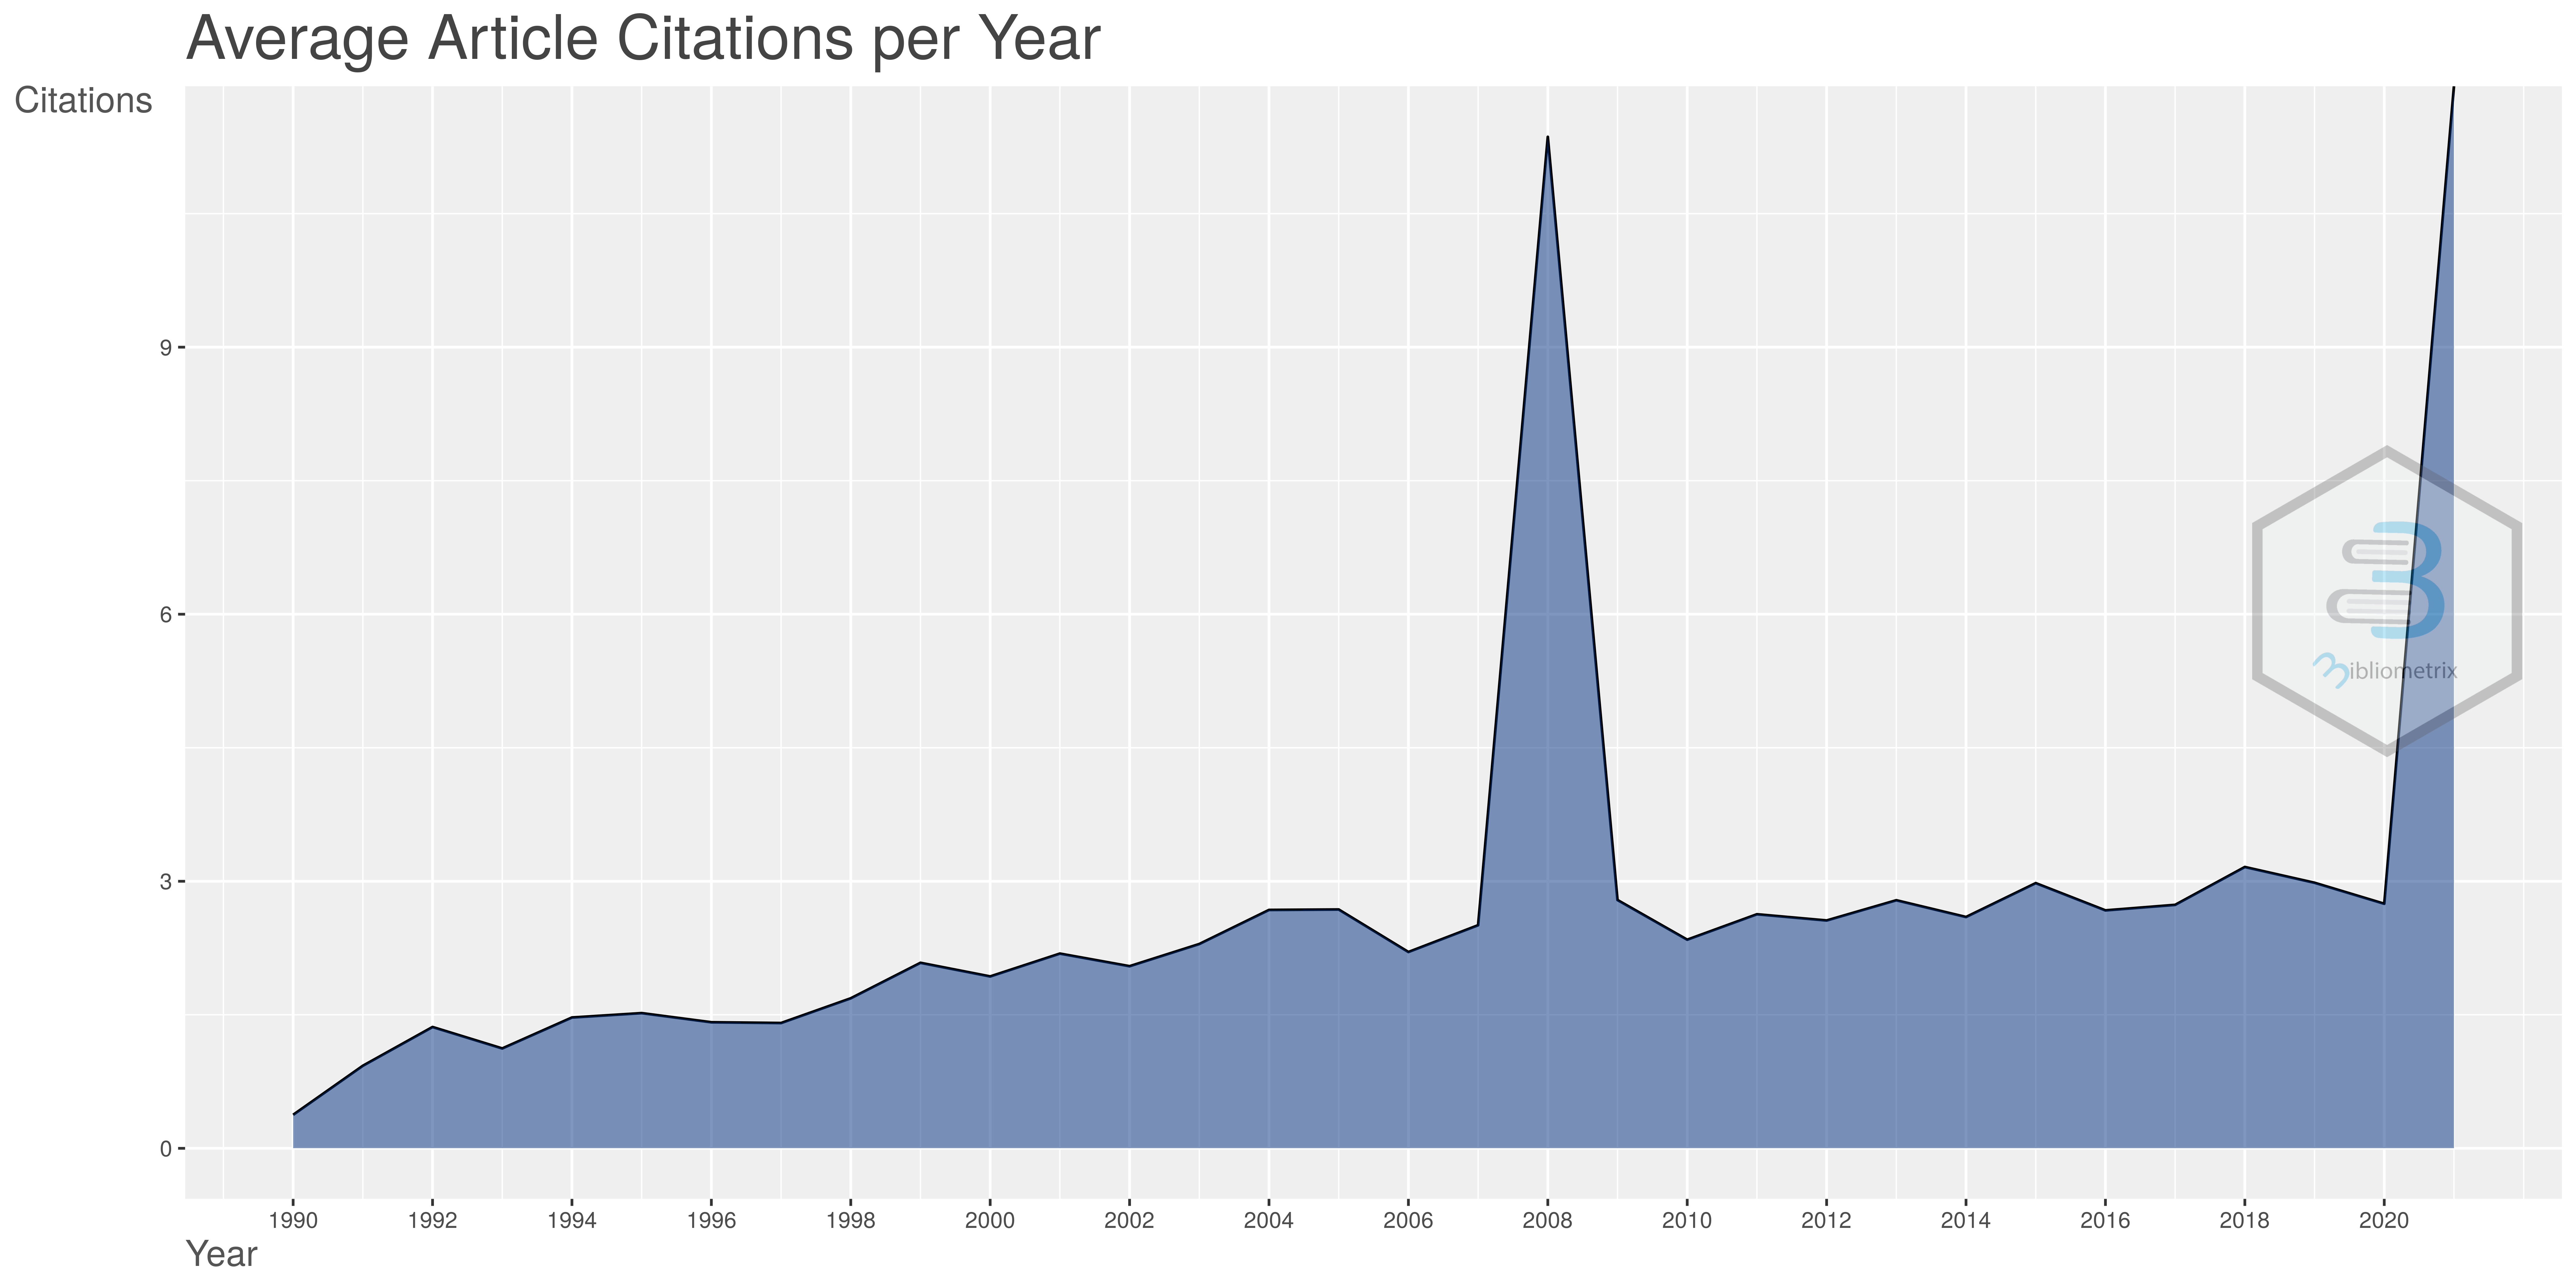
\includegraphics[width=1\textwidth]{experiments/jhcf/PesqBibliogr/SimulacaoMultiagente/WoS-20210803/classico-mais-citacoes/Dataset/AverageArticleCitationPerYear-2021-08-09.png}
    \caption{Evolução das citações ao \dataset\   MASSA@jhcf.}
    \label{fig:evol:anual:citacoes:MASSA@jhcf}
\end{figure}

A figura \ref{fig:evol:anual:citacoes:MASSA@jhcf} apresenta a evolução da média de citações aos 5.787 artigos no \dataset\   MASSA@jhcf. 
Nota-se grande estabilidade na média anual de citações, onde os artigos publicados em 1992 possuem cerca de 2 citações médias, e em 2015 (17 anos depois) o valou alterou-se apenas para três. O pico que aparece no ano de 2008 deve-se, possivelmente, à presença de um artigo do \dataset, publicado em 2008, que possui um número surpreendente grande de citações. \footnote{Note que o cálculo do número  médio de citações, nesse caso, utiliza os valores computados no tag "TC (Times Cited)", já presentes no \dataset\   obtido. Ou seja, o gráfico baseia-se no número de citações globais (externas ao \dataset\   MASSA@jhcf), e não no número de citações locais (citações a um artigo do \dataset\   feitas por alguns dos outros artigos dentro do próprio \dataset).}.

\subsection{Interpretação das Citações}
Mesmo perante um crescimento aproximadamente exponencial no volume de publicações, a ocorrência de um crescimento nas citações médias ao longo dos anos sugere que os artigos do \dataset\   possuem uma tendência de crescimento no tamanho da bibliografia citada, bem como também despertam grande interesse dos cientistas nas demais áreas do conhecimento (já que se trata de citações globais).

\subsection{\textit{Three-Field Plots (Sankey diagram)}}

As \textit{Three-Field Plots (Sankey diagram)} (plotagens do tipo ``Três Campos'') apresentam afinidades entre três conjuntos de atributos agregados que ocorrem no \dataset. Uma plotagem do tipo Sankey busca mostrar os principais fluxos entre diferentes conjuntos de itens. \footnote{Para uma introdução ver \url{https://en.wikipedia.org/wiki/Sankey_diagram}. Para obter detalhes sobre a forma de geração e utilização desse gráfico, inclusive de forma interativa, veja o vídeo em \url{https://www.youtube.com/watch?v=jBb1iha6-sg}.} 

\begin{figure}
    \centering
    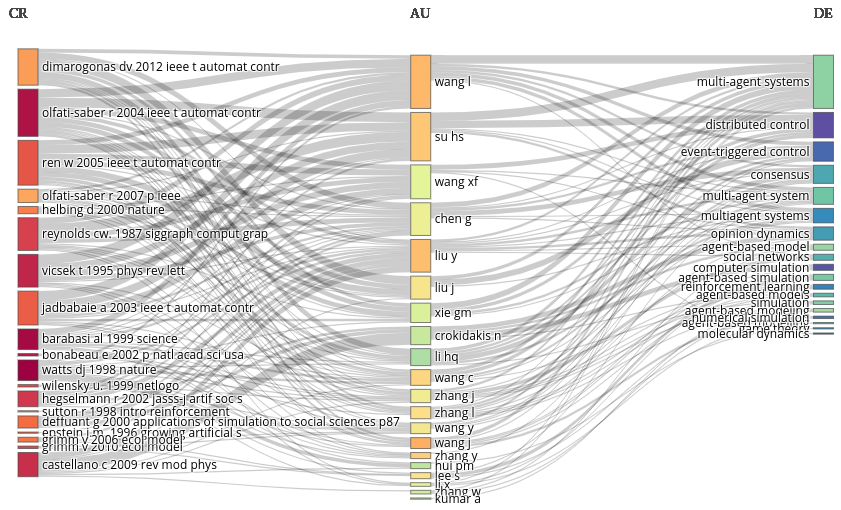
\includegraphics[angle=0,width=1\textwidth]{experiments/jhcf/PesqBibliogr/SimulacaoMultiagente/WoS-20210803/classico-mais-citacoes/Dataset/ThreeFieldPlot-AU-CR-DE-20-20-20.png}
    \caption{Plotagem ``Três Campos'' (Sankey plot) do \dataset\   MASSA@jhcf: 20 Autores, Citações e Palavras-Chave mais proeminentes.}
    \label{fig:MASSA@jhcf:ThreeFieldPlot}
\end{figure}

A figura \ref{fig:MASSA@jhcf:ThreeFieldPlot} apresenta a plotagem do tipo ``Três Campos'' do \dataset\   MASSA@jhcf, vinculando, ao centro, os 20 Autores mais proeminentes (AU), à esquerda, as 20 Citações mais frequentes (CR - Cited Records), e à direita, as 20 Palavras-Chave mais frequentes empregadas pelos autores.

\subsection{Interpretação da figura \ref{fig:MASSA@jhcf:ThreeFieldPlot}}
Os vinte autores mais relevantes, em relação aos artigos mais relevantes citados, e as palavras-chave mais relevantes são aparentemente de origem asiática, mais especificamente chinesa, com base nos sobrenomes. De outra formal, a mesma origem chinesa parece não se aplicar aos trabalhos mais citados, aparentemente europeus ou norte-americanos. Isso sugere estar ocorrendo uma migração recente da produção científica, do ocidente para o oriente. 

Adicionalmente, dentre as palavras-chave (DE) não relacionadas diretamente aos termos de busca, emergem os termos \textbf{distributed control}, \textbf{event-triggered control}, \textbf{consensus} e \textbf{opinion dynamics}. Isso sugere foco das pesquisas por autores de origem chinesa no uso de simulação multiagente voltada à compreensão dos fenômenos de controle social distribuído, formação de consenso e dinâmica da opinião (pública?).

Ainda sobre a interpretação da plotagem da figura \ref{fig:MASSA@jhcf:ThreeFieldPlot}, observa-se que os artigos mais citados encontram-se publicados pelo menos 10 anos atrás, sugerindo que não houve, nos últimos 10 anos, nenhum trabalho que tenha produzido uma mudança de paradigma no tema.
A fim de melhor evidenciar as citações mais relevantes segundo o peso dos autores e palavras-chave, o gráfico da figura \ref{fig:MASSA@jhcf:ThreeFieldPlot:10-20-20} plota apenas as 10 referências citadas, para 20 autores e palavras-chave mais proeminentes.

\begin{figure}
    \centering
    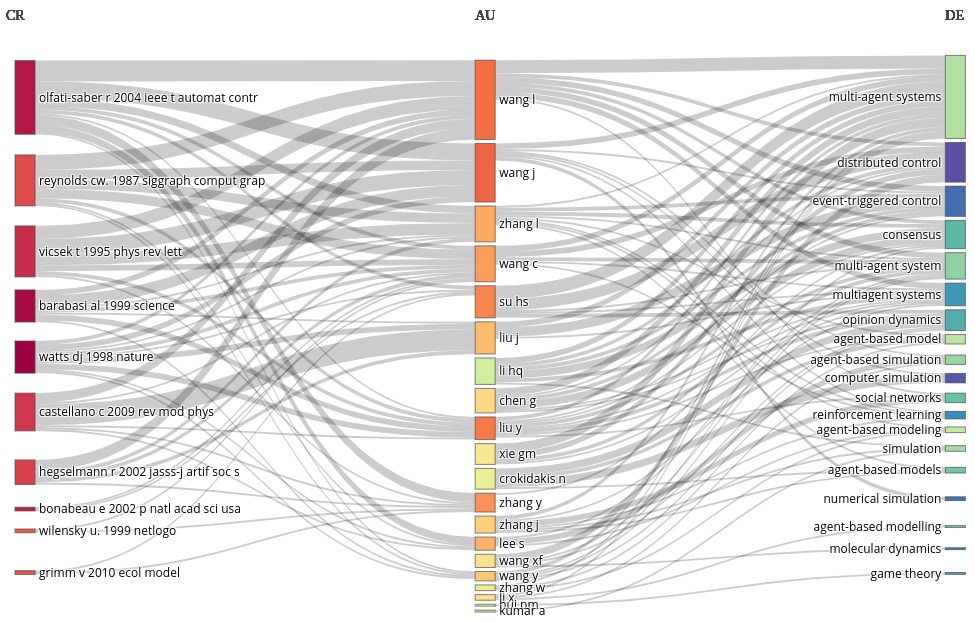
\includegraphics[angle=0,width=1\textwidth]{experiments/jhcf/PesqBibliogr/SimulacaoMultiagente/WoS-20210803/classico-mais-citacoes/Dataset/ThreeFieldPlot-AU-CR-DE-20-10-20.png}
    \caption{Plotagem ``Três Campos'' (Sankey plot) do \dataset\   MASSA@jhcf: 10 Autores, 20 Citações e Palavras-Chave mais proeminentes.}
    \label{fig:MASSA@jhcf:ThreeFieldPlot:10-20-20}
\end{figure}

Breves comentários sobre cada um desses trabalhos serão tratados em seção posterior.

\begin{itemize}
    \item  \cite{olfati-saber_consensus_2004} apresentam discussões teóricas sobre a formação de consenso em sistemas multi-agentes com topologias variáveis;
    \item  \cite{reynolds_flocks_1987} apresenta modelos multi-agentes para simulação gráfica do movimento de rebanhos ou agregados de animais.
    \item \cite{vicsek_novel_1995} analisam a emergência de fenômenos de transição de fase em simulações de de partículas com comportamento autônomo com interação biologicamente motivada.
    \item \cite{barabasi_emergence_1999} investigam a emergência da distribuição livre de escala (\textit{scale-free}\footnote{Ver introdução em \url{https://en.wikipedia.org/wiki/Scale-free_network}.}) em redes que evoluem com base em ligação preferencial.
    \item \cite{watts_collective_1998} exploram o surgimento de redes do tipo mundo pequeno (\textit{small world}\footnote{Ver introdução em \url{https://en.wikipedia.org/wiki/Small-world_network}.}) formadas a partir da reorganização aleatória de redes biológicas, genéticas e outras formas de redes auto-organizadas.
    \item \cite{castellano_statistical_2009} exploram de que forma as técnicas de análise e simulação já usadas na física-estatística podem ser usadas para explicar vários fenômenos sociais, tais como comportamento de multidões, dispersão social, comportamento de multidões etc. Eles apresentam as afinidades entre os dados gerados pelos modelos simulados e dados empíricos obtidos junto a sistemas sociais reais. 
    \item \cite{hegselmann_opinion_2002} exploram a emergência de fenômenos de consenso, polarização e fragmentação da opinião na simulação de sociedades artificiais.
    \item \cite{bonabeau_agent-based_2002} apresenta os potenciais e campos de aplicação da técnicas de simulação baseada em agentes.
    \item \cite{wilensky_netlogo_1999} apresentam a linguagem e ambiente de simulação NetLogo.
    \item \cite{grimm_standard_2006} apresenta o protocolo ODD, proposto para padronizar a descrição de modelos de simulação multiagente.
\end{itemize}

Nenhum desses 10 documentos citados está contido no \dataset\   recuperado.

%\subsection{Análises Bibliométricas: Fontes de Informação}

%\begin{figure}
%    \centering
%    \includegraphics[angle=0,width=1\textwidth]{}
%    \caption{Plotagem ``Três Campos'' (Sankey plot) do dataset MASSA@jhcf: 20 Autores, Citações e Palavras-Chave mais proeminentes.}
%    \label{fig:MASSA@jhcf:ThreeFieldPlot}
%\end{figure}

\section{Refinamento da Coleta de Dados}

No dia 03 de fevereiro de 2022, no decorrer das análises mais refinadas do \dataset\ MASSA@jhcf, identificou-se um grupo de artigos que não se encaixavam no tema de interesse, e que eram voltados para pesquisas no campo da biologia experimental e nanotecnologia. Isso sugeriu que a \query\  de busca precisaria ser reformulada, para excluir artigos que não se enquadrassem na temática desejada.
O conjunto das palavras-chave que refletia essa dissonância ficou evidente na análise da estrutura intelectual do conhecimento, do tipo \textbf{Rede de Co-ocorrências de Palavras-chave}, ilustrada no cluster em roxo, à esquerda da figura \ref{fig:MASSA@jhcf:redecoocorr-150-termos}.

\begin{figure}[htp]
    \centering
    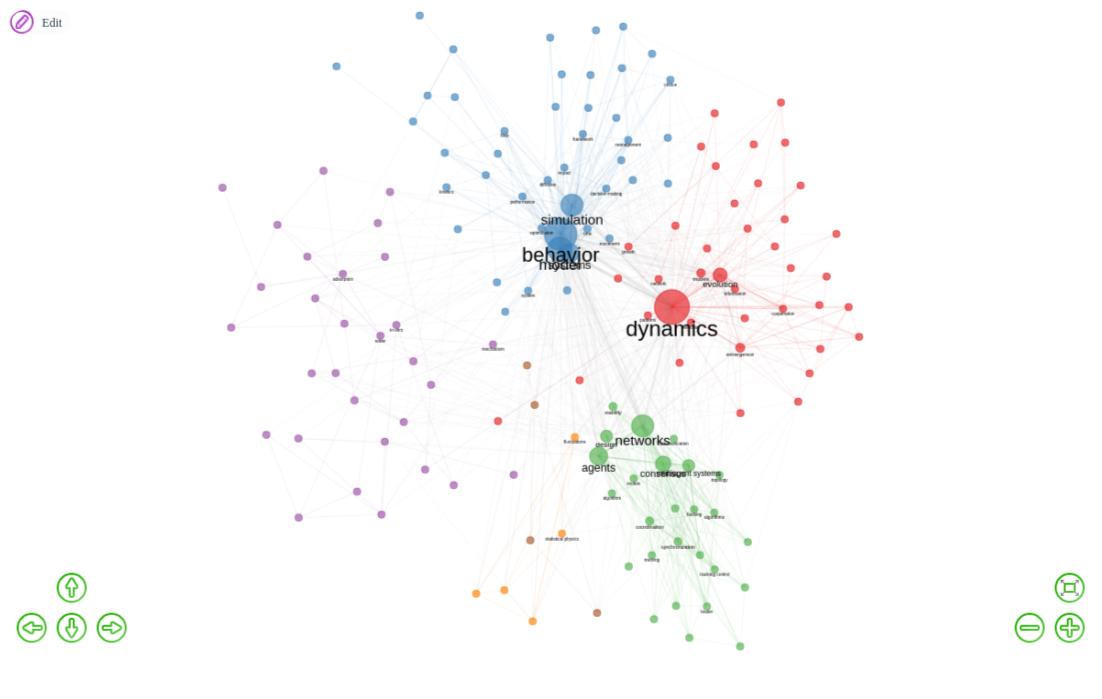
\includegraphics[clip=true,trim={9cm 0cm 7cm 0cm },width=0.6\textwidth]{experiments/jhcf/PesqBibliogr/SimulacaoMultiagente/WoS-20210803/classico-mais-citacoes/Structure-Informetric/Conceptual/Co-occurrence Network-Keywords-Plus-150-termos.png}
    \caption{Rede de co-ocorrência de palavras, com 150 termos, aplicada ao \dataset\   MASSA@jhcf.}
    \label{fig:MASSA@jhcf:redecoocorr-150-termos}
\end{figure}

As seguintes 30 palavras foram identificadas nesse \textit{cluster}:
in-vitro,
adsorption,
mechanism,
water,
force-field,
molecular-dynamics,
binding,
simulations,
nanoparticles,
bubbles,
derivatives,
temperature,
in-vivo,
mathematical-model,
oscillations,
scattering,
cancer,
contrast agents,
expression,
protein,
activation,
delivery,
surface,
removal,
acid,
agent,
reduction,
aqueous-solution,
degradation,
expectations.

Ficou evidente, pela interpretação do significado da maioria desses termos, que tais artigos não tratavam de simulação de fenômenos sociais. Isso sugere que a query está com problemas de precisão, isso é, muitos registros recuperados não atendem à necessidade de informação do pesquisador. 

Algumas dessas palavras foram então escolhidas para servir como indicativas de artigos fora do escopo, e introduzidas a partir da \query\  original, gerando uma nova \query, aprimorada e ilustrada nas linhas 1 a 13 da listagem \ref{query20220203}.

\lstinputlisting[numbers=left,basicstyle=\normalsize\ttfamily,caption={\query\  de busca sobre simulação multiagente de fenômenos socials, com ênfase em métodos experimentais, com escopo negativo de artigos que tratam de experimentos biológicos em vitro.},label=query20220203]
{experiments/jhcf/PesqBibliogr/SimulacaoMultiagente/WoS-20220203/query-Refinada.txt}

Além das justificativas para os termos usados entre as linhas 1 a 9, já descritas em \ref{MASSA:query},  justifica-se na listagem \ref{query20220203}, a inclusão da cláusula \textit{not (
 adsoption or molecular -dynamics or force -field
 or in -vitro or nanopartic* or in -vivo
 or aqueous -solution or protein or surface)}, entre as linhas 10 e 13 da \query, pois elas irão remover artigos não se enquadram no escopo da busca desejada, por usarem uma ou mais desses termos no título, resumo ou palavras-chave do artigo.
 
Usando a nova \query\ de busca, foram recuperados 6.935 documentos, que se encontram em
\url{https://github.com/jhcf/Comput-Experim-20212/experiments/jhcf/PesqBibliogr/SimulacaoMultiagente/ WoS-20220203/wos6935recs.txt}. Isso sugere que aproximadamente 1.000 registros não se enquadravam na necessidade de busca.
Uma nova análise dos dados recuperados é apresentada a seguir.

\section{Nova Análise dos Dados}

\subsection{Nova filtragem de registros}

Sobre os 6.935 documentos recuperados, foram  aplicados os seguintes filtros:
\begin{itemize}
    \item Remoção dos registros de documentos que não são artigos \textit{full paper}, isso é, artigos completos publicados em revistas;
%    \item Remoção dos registros de artigos científicos que não fazem parte do \textit{core} da bibliografa, segundo a Lei de Bradford.
\end{itemize}

Após os filtros aplicados (apenas um)  obteve-se um total de 4.647 registros, que doravante serão chamados de forma coletiva, de \dataset\   MASSA2@jhcf.

\subsection{Análise descritiva do \dataset\   MASSA2@jhcf}

\subsubsection{Dados Sumários Gerais}

\begin{table}[]
    \centering
\csvautotabular[separator=semicolon
%,filter not strcmp={\csvcolii}{}
]{experiments/jhcf/PesqBibliogr/SimulacaoMultiagente/WoS-20220203/Descritiva/MASSA2-Main-Information.csv}
    \caption{Principais dados descritivos do \dataset\   MASSA2@jhcf.}
    \label{tab:MASSA2:Main}
\end{table}

Nota-se, com os resultados da tabela \ref{tab:MASSA2:Main}, que o \dataset\   abrange um período de 32 anos de publicações (1991 a 2022), evidenciando  a publicação dos 4.647 artigos em 1.910 revistas distintas. Esses artigos tem idade média de publicação de 7.8.

Adicionalmente, o \dataset\ apresenta 157.507 referências citadas, com uma média de (157.507/4.647 = ?) 33,89 referências citadas por artigo.

14.229 autores distintos produziram os artigos, com uma média de 3,73 autores por documento.

\subsubsection{}




